\documentclass[10pt]{beamer}
\usefonttheme{professionalfonts,serif}
\def\newblock{\hskip .11em plus .33em minus .07em}
\usepackage[numbers,sort]{natbib}
\renewcommand{\rmdefault}{psbx}
\usepackage[utf8]{inputenc}
\usepackage[T1]{fontenc}
\usepackage{textcomp}
\usepackage{eulervm}

\usetheme{default}           % tips from David Blei
\useinnertheme{circles}
\useoutertheme{infolines}
\setbeamertemplate{headline}{}
\setbeamertemplate{navigation symbols}{}
\setbeamerfont{itemize/enumerate subbody}{size=\normalsize}
\setbeamerfont{itemize/enumerate subsubbody}{size=\normalsize}
\usecolortheme{seahorse}
\setbeamersize{text margin left=2mm,text margin right=2mm}

\graphicspath{{../../figures/}}

\definecolor{mypine}{rgb}{0.05,0.45,0.05}
\definecolor{mycyan}{rgb}{0.0,0.9,0.9}
\newcommand{\Red}{\textcolor{red}}
\newcommand{\Blue}{\textcolor{blue}}
\newcommand{\Green}{\textcolor{mypine}}
\newcommand{\PineGreen}{\textcolor{mypine}}
\newcommand{\Magenta}{\textcolor{magenta}}
\newcommand{\Cyan}{\textcolor{mycyan}}

\newcommand{\N}{\mathcal{N}}
\newcommand{\R}{\mathbb{R}}
\newcommand{\T}{{\scriptsize^{\top}}}
\newcommand{\D}{\mathcal{D}}
\newcommand{\F}{\mathcal{F}}
\newcommand{\E}{\mathbb{E}}
\newcommand{\V}{\mathbb{V}}
\newcommand{\M}{\mathcal{M}}
\newcommand{\KL}{\mathcal{KL}}
\newcommand{\cut}[1]{}
\newcommand{\trace}{\operatorname{trace}}

\newcommand{\bmu}{{\boldsymbol{\mu}}}
\newcommand{\btheta}{\boldsymbol{\theta}}
\newcommand{\bepsilon}{\boldsymbol{\epsilon}}
\newcommand{\balpha}{\boldsymbol{\alpha}}
\newcommand{\bbeta}{\boldsymbol{\beta}}
\newcommand{\bphi}{\boldsymbol{\phi}}
\newcommand{\bPhi}{\boldsymbol{\Phi}}
\newcommand{\bSigma}{\boldsymbol{\Sigma}}
\newcommand{\bpi}{\boldsymbol{\pi}}
\newcommand{\blambda}{\boldsymbol{\lambda}}

\newcommand{\argmax}{\operatorname{argmax}}
\newcommand{\argmin}{\operatorname{argmin}}
\newcommand{\ci}{{\bot\negthickspace\negthickspace\bot}} % conditional indep.
\newcommand{\neigh}{\operatorname{ne}}
\newcommand{\vectr}[2]{  \left[ \!\!\begin{array}{c} #1 \\
      #2 \end{array} \!\!\right]}
\newcommand{\deff}{\stackrel{\mathrm{def}}{=}}
\newcommand{\deldel}[2]{\frac{\partial #1}{\partial #2}}

\newcommand{\maketilde}{\raisebox{0.4ex}{\tiny $\sim$}}
\newcommand{\bfa}{\mathbf a}
\newcommand{\bfb}{\mathbf b}
\newcommand{\bfe}{\mathbf e}
\newcommand{\bff}{\mathbf f}
\newcommand{\bfk}{\mathbf k}
\newcommand{\bfm}{\mathbf m}
\newcommand{\bfn}{\mathbf n}
\newcommand{\bfp}{\mathbf{p}}
\newcommand{\bfs}{\mathbf s}
\newcommand{\bfu}{\mathbf u}
\newcommand{\bfx}{\mathbf x}
\newcommand{\bfy}{\mathbf y}
\newcommand{\bft}{\mathbf t}
\newcommand{\bfv}{\mathbf v}
\newcommand{\bfw}{\mathbf w}
\newcommand{\bfA}{\mathbf A}
\newcommand{\bfI}{\mathbf I}
\newcommand{\bfK}{\mathbf K}


\title{Modelling data}
\author{Carl Edward Rasmussen}
\date{June 29th, 2016}

\begin{document}

\begin{frame}
\titlepage
\end{frame}

\begin{frame}
\frametitle{Origin of a model}

Mathematical models are useful for a number of different purposes.\\

Models may originate from different sources, such as
\begin{description}
\item[first principles] For example, Newtonian mechanics is a model of planetary motion with a high degree of accuracy
\item[observations, data] For example the annual production of timber per hectar of forrest, and its dependency on geographical and climatic factors may be modelled based on \emph{data}.
\end{description}
Most practical models lie somewhere within the  above spectrum, involving both first principles and data.

\emph{Machine learning} is a broad term which covers the theory and practise of mathematical models which to a significant degree rely on data.  
\end{frame}


\begin{frame}
\frametitle{The purpose of a model}

Mathematical models are useful for a number of different purposes.

These include, but are not restricted to
\begin{itemize}
\item making predictions. For example, in a time series model, we may want to predict the futre from the past and the present
\item generalize from the points in the training set to new test cases (interpolation and extrapolation).
\item understading and interpreting statistical relationships in the data
\item evaluating the relative probability of various hypothesis about the data
\item compressing or summarising data.
\end{itemize}

Because there are many uses for models, the usefulness of a model depends on which task we are trying to solve, different models are useful for different purposes.
\end{frame}




\begin{frame}
\frametitle{Assumptions and simplifying assumptions}

Every model relies on (explicit or implicit) assumptions.


There are two types of assumptions
\begin{description}
\item[insights] For example, it might be known that a variable which measures the distance between two points must be non-negative.
\item[simplifying assumptions] We might assume that the response to a drug depends linearly on the dosage within some range. We don't believe that such an assumption is necessarily literaly true, but rather that it is \emph{good enough}, not to distort the uses we have of the model too much.
\end{description}

Often, simplifying assumptions give rise to huge mathematical simplificaitons.

But, the conclusions drawn from a model are conditional on the assumptions being valid.

Practial modelling is therefore always a trade off between model expresivity on one hand and simplicity on the other.
\end{frame}


\begin{frame}
\frametitle{Obervations, parameters and latent variables}

\centerline{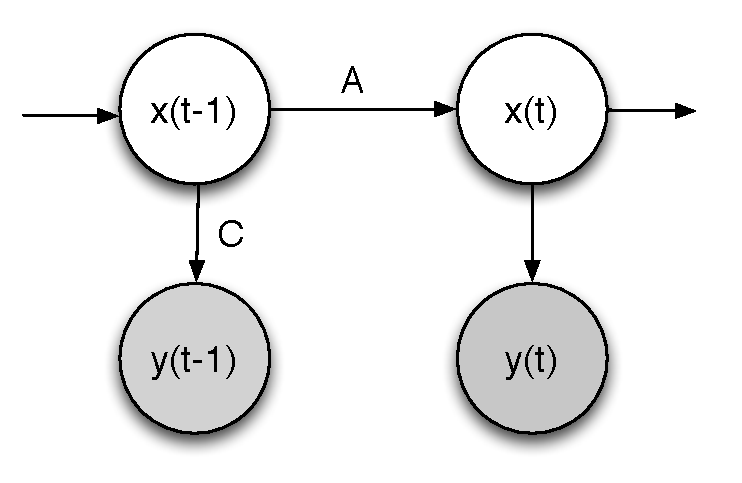
\includegraphics[width=0.4\textwidth]{d1.pdf}}

This time series model is imagined repeated for $t=1,\ldots,T$. It has \Blue{\emph{observations}} $y$ (shaded) for each time point and also \Blue{\emph{unobserved}} or \Blue{\emph{hidden}} or \Blue{\emph{latent variables}} $x$ and two sets of \Blue{\emph{parameters}} $A$ (for transitions) and $C$ (for emissions).\\[1ex]

To use the model we must decide what to do with all unobserved quanteties. Possible options include \Red{\emph{inference}}, \Red{\emph{learning}}, \Red{\emph{estimation}} and \Red{\emph{marginalisation}}.\\[1ex]

Note, that the difference bwteen \Blue{\emph{latent variables}} and \Blue{\emph{parameters}} is that the number latent variables grow with the number of observations (in this case, one for each time point), whereas the number of parameters remains constant.
\end{frame}


\begin{frame}
\frametitle{Practical modelling}

What do we need to do: handle latent variables, handle parameters, model selection
\end{frame}

\begin{frame}
some more about what is the difference between the data and a model. Avoid the term true model.
\end{frame}


\end{document}  